% !TeX program = xelatex
\documentclass[10pt,a4paper]{ctexart} % 设置文章类型，正文字号与纸张大小

% 页面与正文常用宏包
\usepackage[margin=2cm]{geometry} % 设置页面四周页边距
\usepackage{graphicx}             % 插入图片
\usepackage{amsmath}              % 提供cases、aligned等数学公式环境
\usepackage{amssymb}              % 提供\therefore等扩展数学符号
\usepackage{booktabs}             % 提供\toprule、\midrule、\bottomrule三线表命令
\usepackage{float}                % 提供[H]固定图片、表格位置
\usepackage{subcaption}           % 提供subfigure子图环境及子图标题
\usepackage{wrapfig}              % 提供wrapfigure图文环绕环境
\usepackage{fancyhdr}             % 自定义页眉和页脚
\usepackage{hyperref}             % 生成超链接

% 页眉页脚
\pagestyle{fancy}                  % 启用fancyhdr定义的页面样式
\fancyhf{}                         % 清空默认页眉和页脚
\fancyfoot[C]{\thepage}            % 在页脚中央显示页码
\renewcommand{\headrulewidth}{0pt} % 隐藏页眉横线
\renewcommand{\footrulewidth}{0pt} % 隐藏页脚横线

% 超链接
\hypersetup{
  colorlinks=true,                % 使用彩色文字链接，而非带边框的链接
  linkcolor=red,                 % 目录、公式及图表交叉引用的颜色
  filecolor=cyan,                 % 本地文件链接的颜色
  urlcolor=blue,                  % 网址链接的颜色
  pdftitle={交流电路功率因数实验报告},     % 写入PDF文档属性的标题
  bookmarksnumbered=true          % PDF书签显示章节编号
}

% 定义字号命令
\newcommand{\chuhao}{\fontsize{42pt}{63pt}\selectfont}
\newcommand{\xiaochu}{\fontsize{36pt}{54pt}\selectfont}
\newcommand{\yihao}{\fontsize{26pt}{39pt}\selectfont}
\newcommand{\xiaoyi}{\fontsize{24pt}{36pt}\selectfont}
\newcommand{\erhao}{\fontsize{22pt}{33pt}\selectfont}
\newcommand{\xiaoer}{\fontsize{18pt}{27pt}\selectfont}
\newcommand{\sanhao}{\fontsize{16pt}{24pt}\selectfont}
\newcommand{\xiaosan}{\fontsize{15pt}{22.5pt}\selectfont}
\newcommand{\sihao}{\fontsize{14pt}{21pt}\selectfont}
\newcommand{\xiaosi}{\fontsize{12pt}{18pt}\selectfont}
\newcommand{\wuhao}{\fontsize{10.5pt}{15.75pt}\selectfont}
\newcommand{\xiaowu}{\fontsize{9pt}{13.5pt}\selectfont}

% 章节格式
\ctexset{
  section={
    format={\CJKfontspec[AutoFakeBold=2.5]{KaiTi}\sanhao\bfseries}, % 一级标题使用三号加粗楷体
    name={,、},                                                    % 在中文章节序号后添加顿号
    number=\chinese{section},                                      % 一级标题编号使用“一、二、三”形式
    aftername={}                                                   % 取消编号与标题文字之间的空格
  },
  subsection={
    format={\CJKfontspec[AutoFakeBold=2.5]{KaiTi}\sihao\bfseries}, % 二级标题使用四号加粗楷体                                               
  },
  subsubsection={
    format={\CJKfontspec[AutoFakeBold=2.5]{KaiTi}\xiaosi\bfseries}, % 三级标题使用小四加粗楷体
  }
}

\begin{document}

% 封面
\thispagestyle{fancy} % 封面保留底部居中的页码
\fancyfoot[C]{\thepage}
\begin{center}
  \CJKfontspec[AutoFakeBold=2.5]{KaiTi}\bfseries % 封面中文使用楷体并人工加粗，西文同时加粗
  \vspace{0.8cm}
  
\includegraphics[width=8.2cm]{figures/head.png}

  \vspace{0.2cm}
  \xiaochu 
    物理实验报告

  \vspace{3.5cm}
  \begin{minipage}{10.0cm}
    \sanhao
    \makebox[2.6cm][l]{实验名称：}
    \underline{\makebox[7.0cm][c]{交流电路功率因数实验}}\par\vspace{12pt}

    \makebox[2.6cm][l]{实验桌号：}
    \underline{\makebox[7.0cm][c]{19}}\par\vspace{12pt}

    \makebox[2.6cm][l]{指导教师：}
    \underline{\makebox[7.0cm][c]{施博通}}
  \end{minipage}

  \vspace{3.5cm}
  \begin{minipage}{10.0cm}
    \sihao
    \makebox[1.4cm][l]{班级：}
    \underline{\makebox[8.0cm][c]{}}\par\vspace{10pt}

    \makebox[1.4cm][l]{姓名：}
    \underline{\makebox[8.0cm][c]{IllusoryRain}}\par\vspace{10pt}

    \makebox[1.4cm][l]{学号：}
    \underline{\makebox[8.0cm][c]{}}
  \end{minipage}

  \vspace{2.0cm}
  \sihao
    实验日期：
    \underline{\makebox[0.7cm][c]{2026}}年
    \underline{\makebox[0.7cm][c]{9}}月
    \underline{\makebox[0.7cm][c]{23}}日
    星期\underline{\makebox[0.7cm][c]{三}}上午

  \vspace{0.7cm}
  \sihao 
    浙江大学物理实验教学中心
\end{center}

\newpage
\xiaosi\songti\mdseries % 后续正文统一使用小四不加粗的宋体

\section{预习报告（10分）}

  \subsection{实验综述（5分）}
  
    \subsubsection{实验背景}
    交流电功率因数：
     \[
    P=UI\cos\varphi
    \]

    提高交流电功率因数的意义：
    \begin{itemize}
      \item 提高用电利用率
      \item 减少输电线路的损耗
      \item 改善电压质量
      \item 降低用电成本
    \end{itemize}

    \begin{figure}[H]
      \centering
      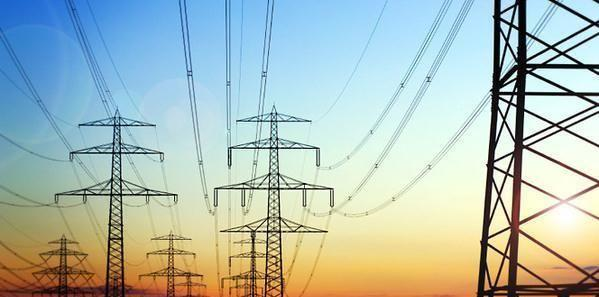
\includegraphics[width=0.6\textwidth]{figures/图1.png}
      \caption{生活中的交流电线}
    \end{figure}

    \subsubsection{交流电功率因数}
    \begin{wrapfigure}{r}{0.25\textwidth}
      \centering
      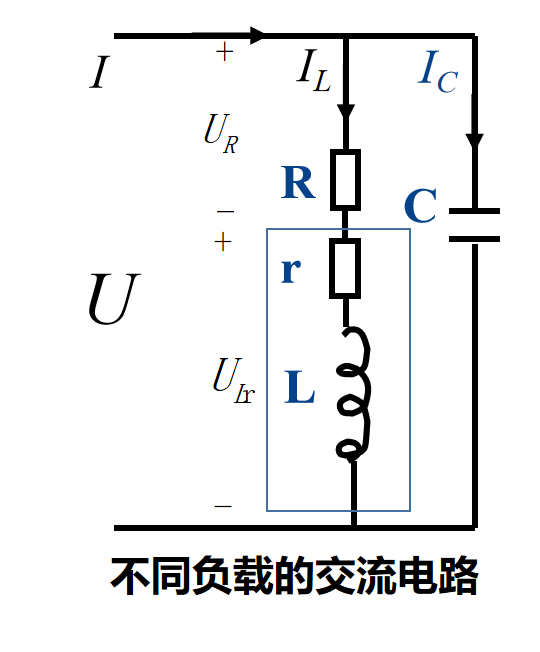
\includegraphics[width=\linewidth]{figures/图2.png}
      \caption{不同负载的交流电路}
    \end{wrapfigure}

    交流电路中的元件有阻性负载、容性负载、感性负载。
    \begin{itemize}
      \item 阻性负载：靠发热来工作的电器都是阻性负载, 阻性负载的特点是，电流和电压同步变化，相位差为“零度”，工作时会产生热量。
      \item 容性负载：电容上电流超前电压90°相位，设想一个电容与电阻串联充电。从充电过程看，总是先有流动电荷（即电流）的积累才有电容上的电压变化，即电流总是超前于电压。
      \item 感性负载：像我们平时用的日光灯等家用电器。电感上电流落后感应电压90°相位。
    \end{itemize}

    如果以电流$I_L$作为相位参考，图3为各物理量之间的相位矢量图。
    由图可见，$I_L$与$U_R$同相；纯电感$L$两端的电压$U_L$比$I_L$超前$\pi/2$。
    合成电压$U$的大小为总电压的幅值，$\varphi$为 $I_L$ 落后于$U$的相位角。

    对应提高电感性电路的功率因数，常用的方法就是在靠近感性负载端并联电容器，其电路图如图4所示，
    由相量图可知原感性负载电流滞后于电压$\varphi$，当并联电容以后，只要电容的大小选择得当，
    就可以使并联电容以后的总电流小于原来电感中的电流，使$\varphi'<\varphi$，使功率因数得到提高。 

    \begin{figure}[H]
      \centering
      \begin{minipage}{0.4\textwidth}
        \centering
        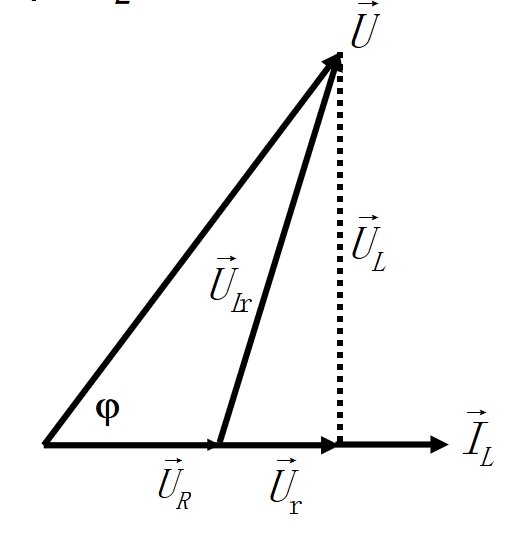
\includegraphics[width=\linewidth]{figures/图3.png}
        \caption{相位矢量图}
      \end{minipage}
      \hfill
      \begin{minipage}{0.4\textwidth}
        \centering
        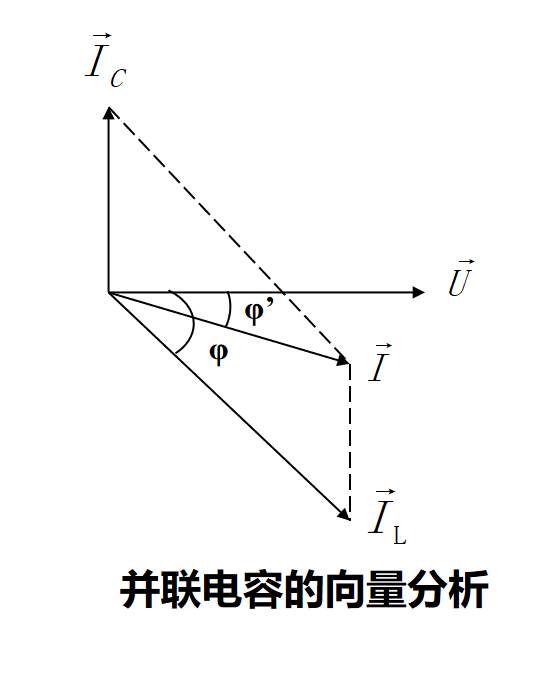
\includegraphics[width=\linewidth]{figures/图4.png}
        \caption{并联电容的向量分析}
      \end{minipage}
    \end{figure}

    \subsubsection{日光灯管的工作原理}
    日光灯电路是日常照明电路中一种较为经济的照明电路，也是一种典型的电感性负载电路，它主要由灯管、镇流器、启辉器组成。

    镇流器是一个带铁芯的自感线圈，自感系数很大。

    启辉器主要是一个充有氖气的小氖泡，里面装有两个电极，一个是静触片，一个是由两个膨胀系数不同的金属制成的U型动触片
    （双层金属片——当温度升高时，因两层金属片的膨胀系数不同，且内层膨胀系数比外层膨胀系数高，所以动触片在受热后会向外伸展）。

    \begin{figure}[H]
      \centering
      \begin{minipage}{0.35\textwidth}
        \centering
        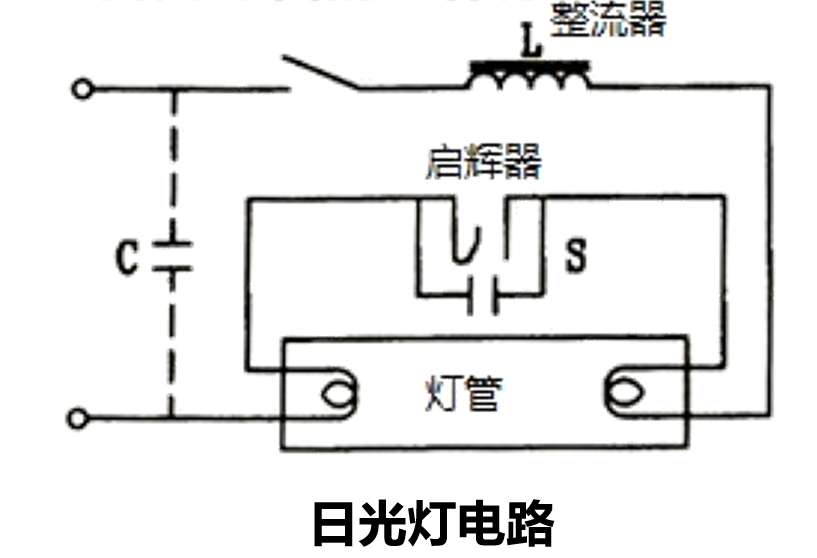
\includegraphics[width=\linewidth]{figures/图5.png}
        \caption{日光灯电路}
      \end{minipage}
      \hfill
      \begin{minipage}{0.35\textwidth}
        \centering
        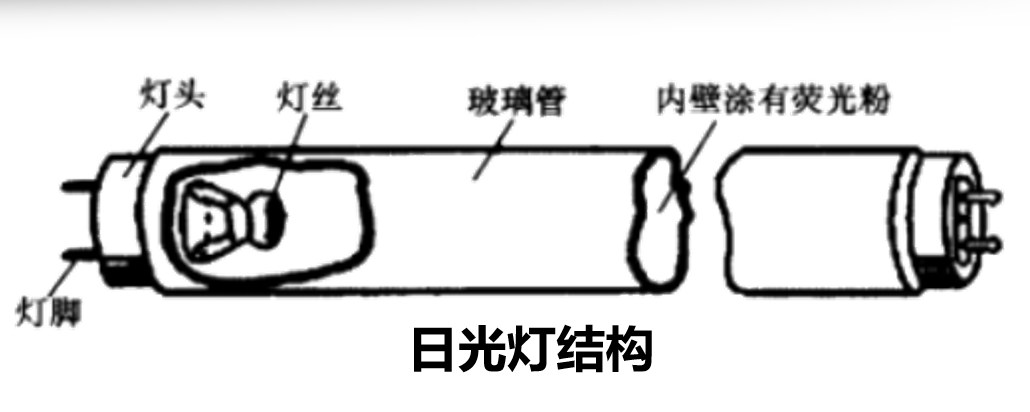
\includegraphics[width=\linewidth]{figures/图6.png}
        \caption{日光灯结构}
      \end{minipage}
      \hfill
      \begin{minipage}{0.15\textwidth}
        \centering
        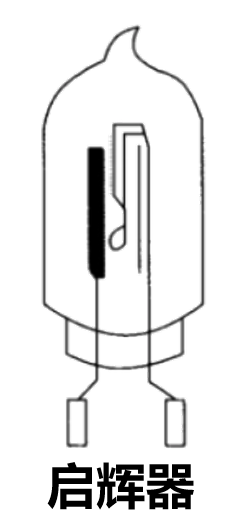
\includegraphics[width=\linewidth]{figures/图7.png}
        \caption{启辉器}
      \end{minipage}
    \end{figure}

  \subsection{实验重点（3分）}
  \begin{enumerate}
    \item 理解功率因数的物理意义；
    \item 掌握提高电感性电路功率因素的方法；
    \item 熟悉日光灯的工作原理，掌握测量日光灯功率的方法。
  \end{enumerate}

  \subsection{实验难点（2分）}
  \begin{enumerate}
    \item 理解并联电容器对交流电路功率因数的影响；
    \item 分析并联电容后电路电流的变化；
    \item 准确测量$U$、$I$和$P$，计算不同电容量下的功率因数并分析其变化规律。
  \end{enumerate}

\section{实验操作与原始数据（50分）}
% 填写自己的实验数据图

\section{结果与分析（30分）}

  \subsection{数据处理与结果（20分）}  
  把原始数据代入公式
  \[
  P=UI\cos\varphi
  \]
  计算得到频率分别为45,50,55Hz时的功率因数$\cos\varphi$, 转化以下表格:
  \begin{table}[H]
    \centering
    \caption{50Hz时不同电容下的功率因数}
    \begin{tabular}{ccccccccc}
      \toprule
      $C/\mu\mathrm{F}$ & 0 & 1 & 2 & 3 & 4 & 5 & 6 & 7 \\
      \midrule
      $I/\mathrm{A}$ & 0.313 & 0.249 & 0.195 & 0.150 & 0.125 & 0.127 & 0.158 & 0.203 \\
      $U/\mathrm{V}$ & 219.3 & 219.7 & 220.0 & 220.0 & 219.8 & 219.2 & 219.0 & 219.0 \\
      $P/\mathrm{W}$ & 24.2 & 24.6 & 24.9 & 25.1 & 25.1 & 24.6 & 24.5 & 24.7 \\
      $\cos\varphi$ & 0.353 & 0.450 & 0.580 & 0.761 & 0.914 & 0.884 & 0.708 & 0.556 \\
      \bottomrule
    \end{tabular}
  \end{table}

  \begin{table}[H]
    \centering
    \caption{45Hz时不同电容下的功率因数}
    \begin{tabular}{ccccccccc}
      \toprule
      $C/\mu\mathrm{F}$ & 0 & 1 & 2 & 3 & 4 & 5 & 6 & 7 \\
      \midrule
      $I/\mathrm{A}$ & 0.389 & 0.336 & 0.284 & 0.238 & 0.200 & 0.174 & 0.164 & 0.172 \\
      $U/\mathrm{V}$ & 219.6 & 219.8 & 220.0 & 220.3 & 220.5 & 220.7 & 220.8 & 220.6 \\
      $P/\mathrm{W}$ & 30.8 & 30.8 & 31.1 & 31.2 & 31.4 & 31.5 & 31.6 & 31.7 \\
      $\cos\varphi$ & 0.361 & 0.417 & 0.498 & 0.595 & 0.712 & 0.820 & 0.873 & 0.835 \\
      \bottomrule
    \end{tabular}
  \end{table}

  \begin{table}[H]
    \centering
    \caption{55Hz时不同电容下的功率因数}
    \begin{tabular}{ccccccccc}
      \toprule
      $C/\mu\mathrm{F}$ & 0 & 1 & 2 & 3 & 4 & 5 & 6 & 7 \\
      \midrule
      $I/\mathrm{A}$ & 0.267 & 0.198 & 0.141 & 0.105 & 0.113 & 0.154 & 0.213 & 0.272 \\
      $U/\mathrm{V}$ & 219.0 & 219.5 & 219.3 & 218.8 & 218.5 & 218.4 & 218.4 & 218.4 \\
      $P/\mathrm{W}$ & 21.1 & 21.3 & 21.3 & 21.3 & 21.4 & 21.3 & 21.5 & 21.6 \\
      $\cos\varphi$ & 0.361 & 0.490 & 0.689 & 0.927 & 0.863 & 0.633 & 0.462 & 0.364 \\
      \bottomrule
    \end{tabular}
  \end{table}

  拟合为以下图像：
  \begin{figure}[H]
    \centering
    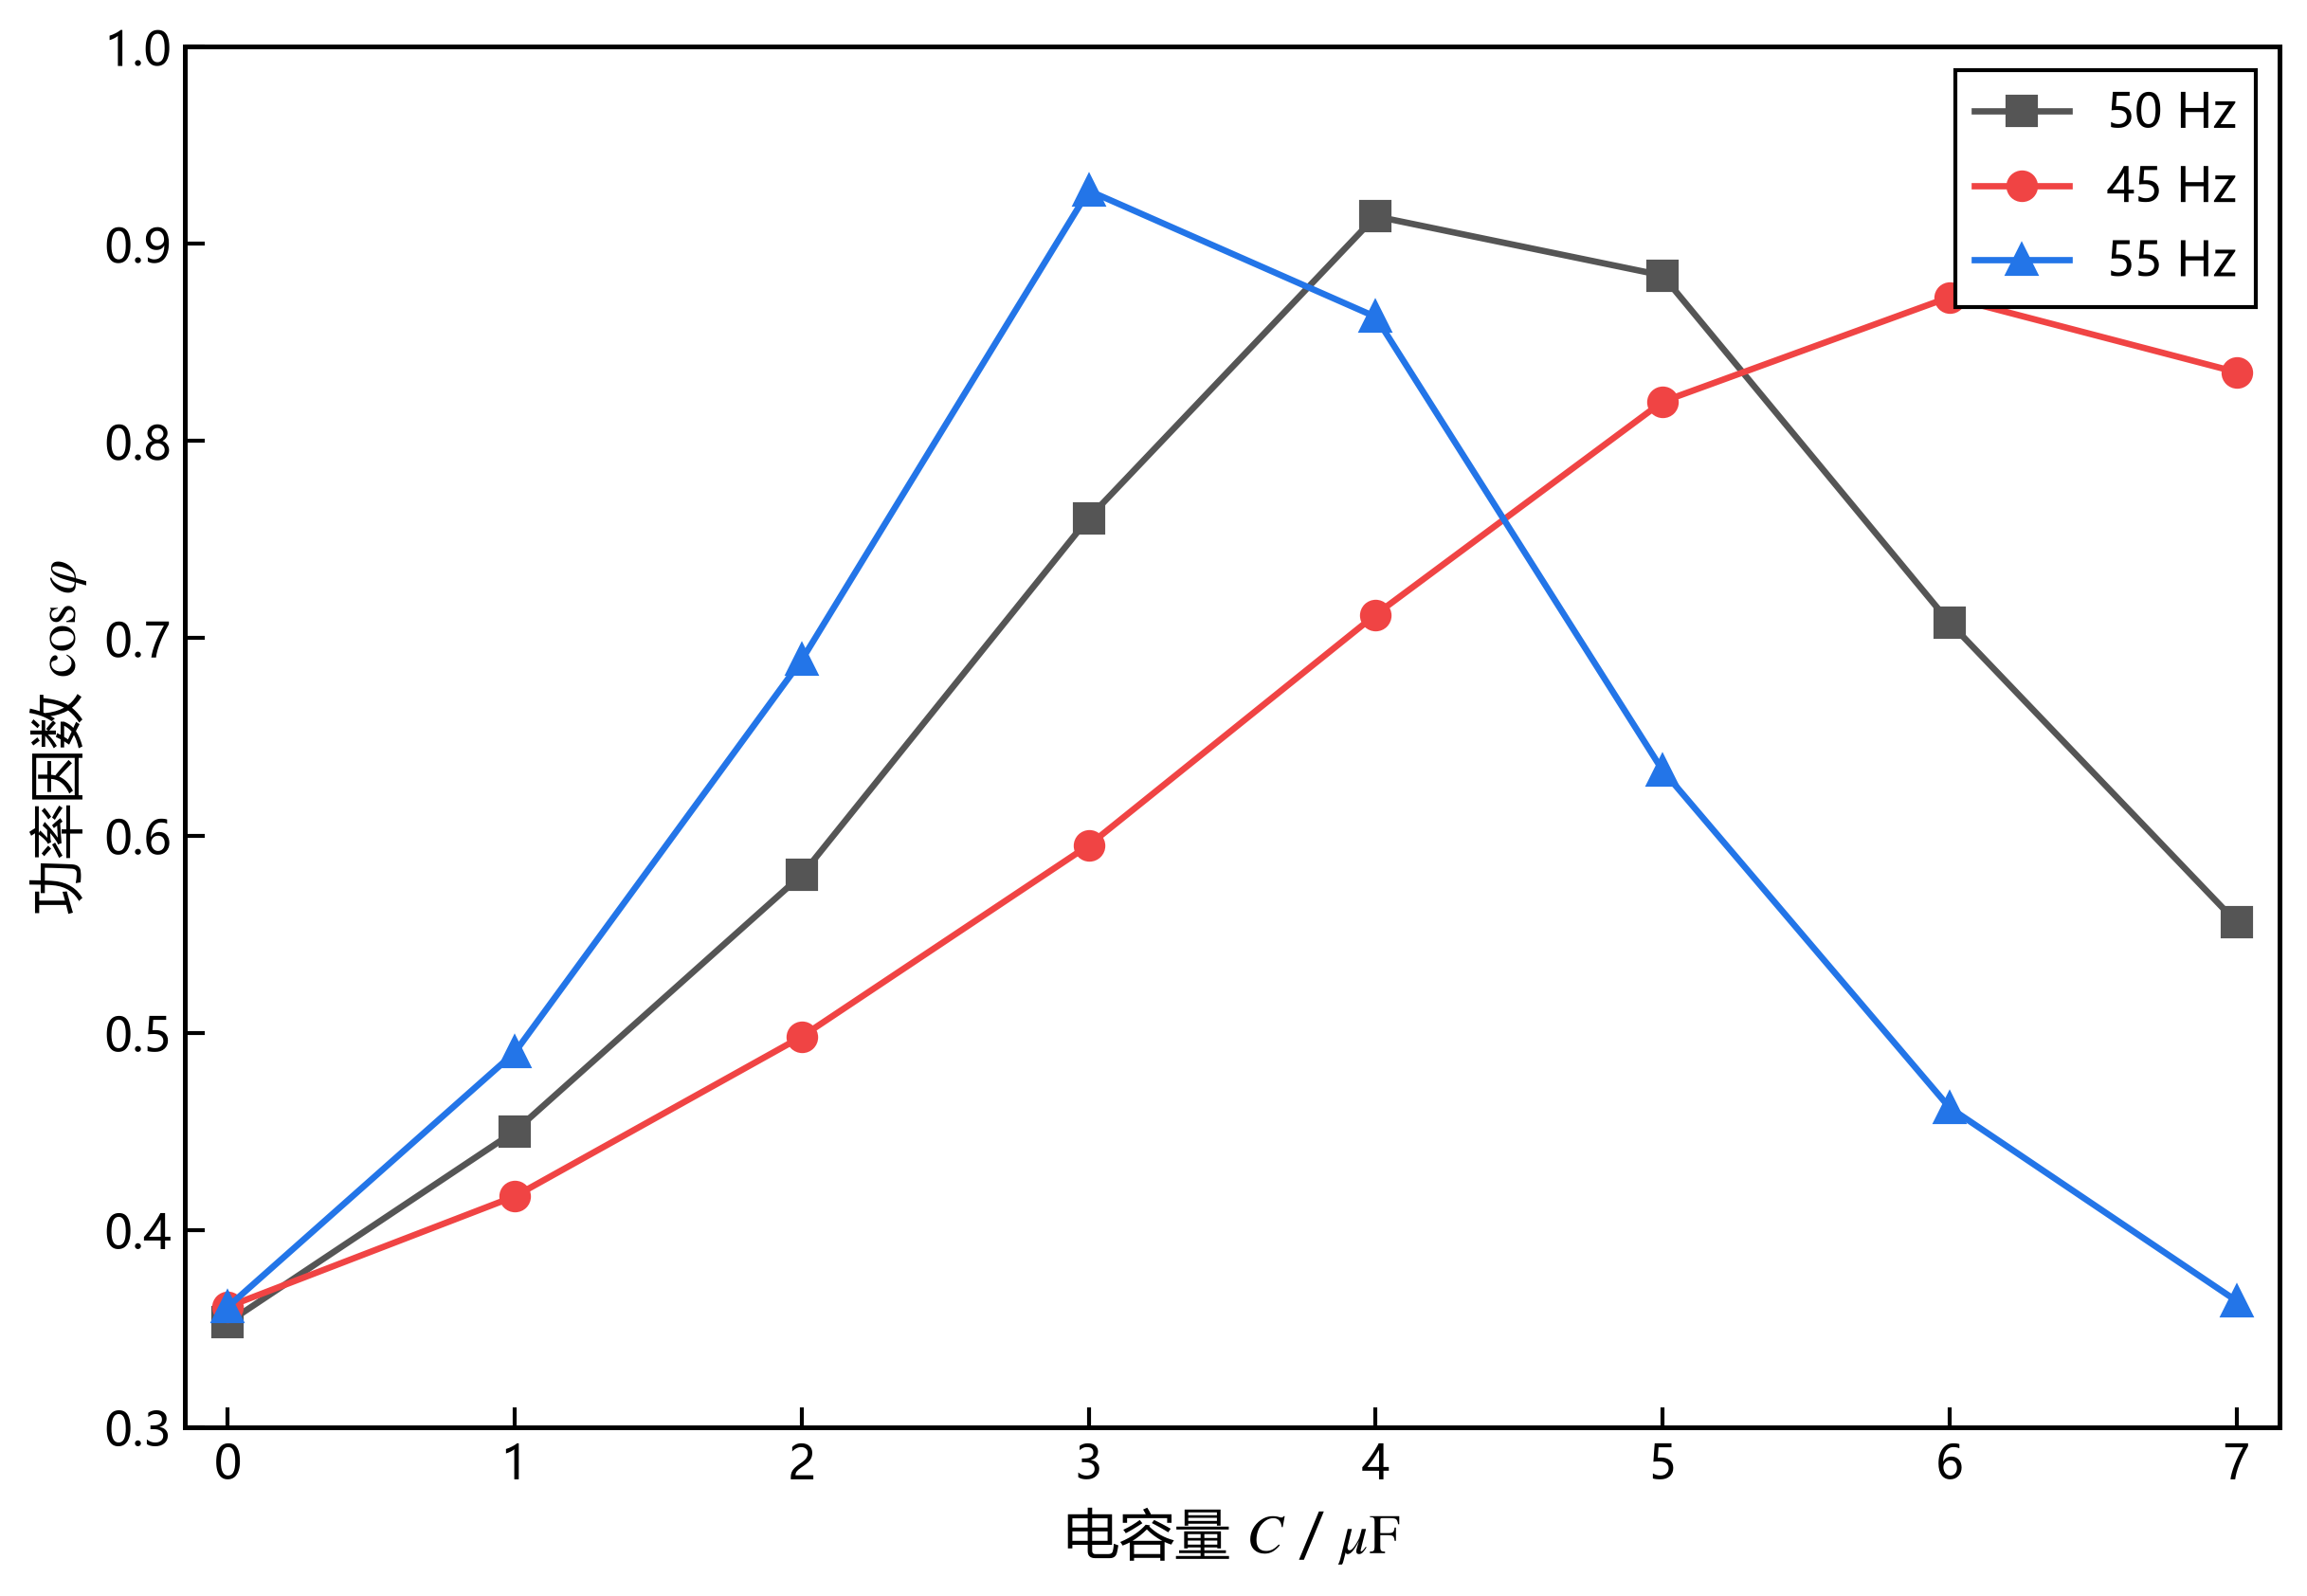
\includegraphics[width=0.7\textwidth]{figures/图10.png}
    \caption{不同频率下功率因数与电容量的关系}
  \end{figure}

  由表格及折线图可以看出，在三种频率下，随着并联电容量逐渐增大，功率因数均呈现先增大后减小的变化趋势，而电路总电流则呈现先减小后增大的变化趋势。
  不同频率下，功率因数达到最大值时所对应的电容量不同：在本实验测量范围内，45、50、55Hz时分别约为$6$、$4$、$3\,\mu\mathrm{F}$。

  在$50\,\mathrm{Hz}$条件下，未接入电容时，电路总电流为$0.313\,\mathrm{A}$，功率因数仅为$0.353$，说明电路中存在较大的无功电流分量。
  随着并联电容量增大，电流逐渐减小，功率因数逐渐提高。
  当电容量为$4\,\mu\mathrm{F}$时，总电流达到测量中的最小值$0.125\,\mathrm{A}$，功率因数达到最大值$0.914$。
  继续增大电容量后，功率因数下降，总电流重新增大；当电容量为$7\,\mu\mathrm{F}$时，功率因数降至$0.556$，电流增至$0.203\,\mathrm{A}$。

  在$45\,\mathrm{Hz}$ 条件下，未接入电容时，总电流为$0.389\,\mathrm{A}$，功率因数为$0.361$。随着电容量增加，功率因数持续提高，电流逐渐减小。
  当电容量为$6\,\mu\mathrm{F}$ 时，功率因数达到测量中的最大值$0.873$，总电流降至最小值$0.164\,\mathrm{A}$。
  当电容量进一步增至$7\,\mu\mathrm{F}$时，功率因数降至$0.835$，总电流回升至$0.172\,\mathrm{A}$，表明继续增大电容量已不能进一步改善补偿效果。

  在$55\,\mathrm{Hz}$ 条件下，未接入电容时，总电流为$0.267\,\mathrm{A}$，功率因数为$0.361$。
  当电容量增加至$3\,\mu\mathrm{F}$时，功率因数达到测量中的最大值$0.927$，总电流降至最小值$0.105\,\mathrm{A}$。
  此后随着电容量继续增大，功率因数逐渐下降，总电流逐渐增大；当电容量为$7\,\mu\mathrm{F}$时，功率因数降至$0.364$，总电流增至$0.272\,\mathrm{A}$，略高于未补偿时的电流。

  上述变化与并联电容补偿的原理一致。感性负载的电流滞后于电压，而电容支路电流超前于电压。
  适当并联电容可抵消一部分感性无功电流，减小电源提供的总电流，使功率因数提高，电路整体特性向阻性靠近。
  电容量过大时则可能出现过补偿，剩余的容性无功电流增大，使总电流重新上升、功率因数下降。因此，并联电容并非越大越好，应根据负载和工作频率选择合适的电容量。

  对比三组数据可知，在本实验条件下，频率越高，测得的最佳补偿电容量越小。这是因为频率变化既会影响感性负载的无功需求，
  也会影响电容支路的电流，因此不能将某一频率下的最佳电容量直接用于其他频率。
  此外，三组数据的最大功率因数均小于$1$，说明补偿后仍未达到完全阻性的状态。
  由于电容量以$1\,\mu\mathrm{F}$为步长取值，上述最佳电容量仅对应已测数据点，其更精确的位置还需通过加密测量确定。

  \subsection{误差分析（10分）}
  本实验的误差主要来自以下几个方面：
  \begin{enumerate}
    \item 仪表误差：电压表、电流表和功率表的精度及读数波动会影响$\cos\varphi=P/(UI)$的计算结果。
    \item 电容容量偏差：电容器的实际容量与标称值存在差异，使实际补偿效果与预期不完全一致。
    \item 工作状态变化：电源电压、频率的波动以及日光灯和镇流器温度的变化，均可能引起电流和功率变化。应在电路稳定后记录数据。
    \item 取样与数据处理：电容量以$1\,\mu\mathrm{F}$为步长取值，限制了最佳补偿电容量的确定精度；读数记录和小数舍入也会引入误差。
  \end{enumerate}

  实验测得的实际电容如下：
  \begin{table}[H]
    \centering
    \caption{实际电容}
    \begin{tabular}{ccccccc}
      \toprule
      $C/\mu\mathrm{F}$ & 1A & 1B & 1C & 2A & 2B & 2C \\
      \midrule
      $C/\mu\mathrm{F}$ & 0.9023 & 0.9291 & 1.0123 & 1.7788 & 1.8338 & 1.8702 \\
      \bottomrule
    \end{tabular}
  \end{table}

\section{实验探讨与思考题（10分）}

  \subsection{实验探讨}
  通过本实验，我理解了并联电容提高功率因数的原理，认识到电容并非越大越好，且最佳补偿容量随频率变化。
  我同时也体会到了准确读数、记录和合理处理数据的重要性。

  \subsection{思考题}

    \subsubsection{提高功率因数的意义何在？为什么并联电容能提高功率因数？并联电容是否越大越好？}
    答：在有功功率和电源电压一定时，提高功率因数可以减小线路电流，从而降低线路损耗和电压降，提高供电设备的利用率。
    日光灯电路含有镇流器，属于感性负载，其电流滞后于电压。
    并联电容器后，电容支路产生超前于电压的电流，可抵消一部分感性无功电流，使电源提供的总电流减小，功率因数提高。
    电容并非越大越好：补偿过度后，电路会由感性变为容性，总电流重新增大，功率因数反而下降。

    \subsubsection{在实验中，随着电容增加，电路总电流的变化规律为由大变小再变大，试分析原因。}
    答：并联电容后，电源电流是负载电流与电容电流的相量和。设负载电流的有功分量为$I_{\mathrm P}$、感性无功分量为$I_{\mathrm Q}$，电容电流约为$I_{\mathrm C}=\omega CU$，则
    \[
    I=\sqrt{I_{\mathrm P}^{\,2}+(I_{\mathrm Q}-I_{\mathrm C})^{2}}。
    \]
    随着电容$C$增加，$I_{\mathrm C}$逐渐增大，起初抵消越来越多的感性无功分量，总电流减小；当两者接近相等时，总电流达到最小；
    继续增大电容则造成过补偿，容性无功分量增大，总电流又上升。

    \subsubsection{在进行功率因数补偿时，本实验采用并联电容器的方法，为什么不采用串联电容器的方法？}
    答：并联电容器可以提供超前的无功电流，减少电源需要提供的感性无功电流，同时负载仍基本承受原来的电源电压，因而适合在不明显改变日光灯工作状态的条件下进行功率因数补偿。
    若将电容器串联接入，电容会改变电路的总阻抗以及灯管、镇流器上的电压和电流，影响日光灯的启动与正常工作；在某些参数下还可能出现串联谐振及局部过电压。
    因此，本实验不采用串联电容器。

\vspace*{\fill} % 使下面内容在页面底部显示
\noindent
\begin{minipage}{\textwidth}
  注意事项：

  \begingroup
    \setlength{\leftskip}{2em} % 1--4整体向右缩进两个汉字宽度
    1. 用PDF格式上传“实验报告”，文件名：学生姓名+学号+实验名称+周次。

    2. “实验报告”必须递交在“学在浙大”本课程内对应实验项目的“作业”模块内。

    3. “实验报告”成绩必须在“浙江大学物理实验教学中心网站”-“选课系统”内查询。

    4. 教学评价必须在“浙江大学物理实验教学中心网站”-“选课系统”内进行，学生必须进行教学评价，才能看到实验报告成绩，教学评价须在本次实验结束之后3天内进行。\par
  \endgroup

  \begin{center}
    {\CJKfontspec[AutoFakeBold=2.5]{SimSun}\bfseries 浙江大学物理实验教学中心制}
  \end{center}
\end{minipage}

\end{document}
